\documentclass[10pt,a4paper]{article}
\usepackage[margin=2.2cm]{geometry}
\usepackage{amsmath,amssymb}
\usepackage{graphicx}
\usepackage{booktabs}
\usepackage{array}
\usepackage{rotating}
\usepackage[hidelinks]{hyperref}
\usepackage{parskip}
\setlength{\parindent}{0pt}

\newcommand{\msgu}{\ensuremath{\lVert G\rVert/\lVert S_w\rVert}}
\newcommand{\qbar}{\ensuremath{\bar q}}
\newcommand{\pmm}[2]{\ensuremath{#1 \pm #2}}

\title{Causal Probabilistic Transformer:\\ experimental report, 2026-08-09 -- 2026-08-11}
\author{Viktor Beliakov\\ \small ShanghaiTech University, NLP group of Prof.\ Kewei Tu}
\date{2026-08-11}

\begin{document}
\maketitle

\begin{abstract}
\noindent The causal PT decoder was implemented from scratch, validated against the worked
example of the technical note digit for digit, and trained on PTB. Best replicated result:
validation perplexity \pmm{250.69}{2.32}, test \pmm{229.31}{2.62} (three seeds), against a
unigram baseline of 688.82, a GPT baseline of 115.43 and a Looped-Transformer baseline of
126.46 on the identical pipeline and scored token set --- at 16{,}448 non-embedding
parameters against the GPT's 1{,}237{,}440. This document is the full record: every
experiment, every number, the failed diagnoses (kept and marked \textsc{superseded}), the
corrections log, and the reproduction map. Every number is sourced from a run JSON, a slurm
log, or a checkpoint inspection. Single-seed results are labelled as such throughout.
Repository: \url{https://github.com/b3ly4ck/probabilistic-transformer-experiments}
(commits \texttt{7985174}\,\ldots\,\texttt{7f70e5f}).
\end{abstract}

\section{Executive summary}

\begin{table}[h]\centering\small
\resizebox{\textwidth}{!}{%
\begin{tabular}{lllll}
\toprule
model & val ppl & test ppl & emb / non-emb params & seeds\\
\midrule
\textbf{Causal PT, best} ($d{=}32,h{=}2,\alpha_Z{=}0.25$, frozen $b$) & \textbf{\pmm{250.69}{2.32}} & \textbf{\pmm{229.31}{2.62}} & 330{,}000 / 16{,}448 & 3\\
Causal PT, best 2$\times$2 cell (floor 0.5 + $G_t$) & \pmm{247.66}{5.36} & \pmm{225.52}{5.46} & 330{,}000 / 18{,}496 & 3\\
Looped Transformer (1 shared block $\times$ 4) & 126.46 & 117.93 & 1{,}610{,}240 / 309{,}600 & 1\\
GPT (nanoGPT, 4 layers) & 115.43 & 107.16 & 1{,}610{,}240 / 1{,}237{,}440 & 1\\
unigram baseline & 688.82 & --- & --- & exact\\
\bottomrule
\end{tabular}}
\end{table}

The PT is $2.17\times$ worse than the GPT on validation at $75\times$ fewer non-embedding
parameters. It cannot currently be given a comparable budget: without damping it collapses
above $d=24$ labels and above $h=2$ channels, and with damping the $d$-ladder is
non-monotone (open). The matched-budget comparison the research plan requires therefore does
not exist yet; the honest object is the trade curve of Fig.~\ref{fig:trade}, which is what
\S22.3 of the technical note anticipated.

Three mechanisms were established.

\textbf{(1) The message/unary balance decides learning, and the transition is visible within
a run.} The scalar $\msgu$ (head message against word unary in the content stream) separates
every run that learns from every run that lands on the unigram, across ${\sim}30$ PTB runs
without exception. In run 940844 the model sits at the unigram for 2000 steps and validation
perplexity drops $703.6 \to 539.0$ at the very evaluation where \msgu{} first enters the
healthy range; in run 940848 an excursion out of the range at steps 1500--2000 coincides
with perplexity \emph{reverting} $516 \to 694$, then resuming its fall when the scalar
re-enters. The dependence is two-sided (Figs.~\ref{fig:phase},~\ref{fig:excursion}).

\textbf{(2) A step size below 1 on the label update (Wu \& Tu App.~B.1) breaks the runaway
loop and opens $d=32$.} The loop $\qbar \to B \to G \to \qbar$ explodes at $d=32$ (\msgu{}
$2.88 \to 20.57$ between steps 500 and 1000); $\alpha_Z=0.25$ damps it and takes validation
perplexity from 315.46 (the $d{=}16$ ceiling) to \pmm{250.69}{2.32}. This is the largest
single gain of the session and is replicated over three seeds. $\alpha_Z=0.5$ is not enough
(531.10, single seed).

\textbf{(3) The B.3.3 global head dies by a symmetry trap and revives only when treated
unlike the other factors.} Under uniform initialisation and a shared L2, the rows of $B'$
collapse to one row replicated $m$ times (row spread $0.0197 \to 0.0037$ while within-row
structure stays $0.90$); the gradient argument is two lines (\S\ref{sec:gt}). With
asymmetric initialisation and no L2 on $B'$ the head carries half the total message and
improves an undamped $d=24$ by 7.4\,\%. On the damped record it \emph{costs} 7.7\,\% and
doubles the seed variance. Both readouts defeat it for different reasons: under the exact
readout its contribution is a constant by construction (measured to $10^{-12}$); under MFVI
it is degenerate by optimisation unless specially treated.

\textbf{Interaction claim, withdrawn.} On single seeds, $G_t$ + a raised cosine floor beat
the record (241.89 vs 248.29) while each intervention alone was worse --- an apparent
interaction. Replication over three seeds gives \pmm{247.66}{5.36} against \pmm{250.69}{2.32}:
a 1.2\,\% difference against overlapping ranges. The single-seed record of 241.89 is
withdrawn; the defensible number is the damped $d=32$ figure above.

\section{Setup}

\textbf{Data.} PTB word level, Mikolov preprocessing, one sentence per line,
\texttt{<eos>} appended. Vocabulary from train: 10{,}000 types. Tokens: train 929{,}589,
valid 73{,}760, test 82{,}430. Fixed-length blocks of 64 tokens from the joined stream,
identical for every model.

\textbf{Unigram floor.} ML unigram from train counts (no smoothing; the vocabulary is built
from train), scored on the identical token set (deterministic non-overlapping validation
blocks, first slot dropped): val \textbf{688.82} (687.45 with slot 0). The pre-registered
gate was half of it, 344.41.

\textbf{Evaluation protocol.} PT's $\mathrm{logits}[:,t]$ predicts $w_t$ from $w_{<t}$
(slot 0 from ROOT alone). The GPT wrapper runs the backbone on $\mathrm{idx}[:, :-1]$ and
shifts its output right by one slot, so both models answer $p(w_t \mid w_{<t})$; slot 0 of
the GPT is zeros and its loss asserts it is never scored. \texttt{ignore\_first}=1
everywhere makes the scored token sets identical (asserted by a test). Evaluation is
deterministic (fixed blocks, whole split); train perplexity is measured on a fixed 20-batch
slice the same way. The context probe (prefix ablation) compares the last-slot predictive
distribution under the true prefix, a shuffled prefix, and a constant prefix (KL, max
$|\Delta\mathrm{logit}|$, argmax agreement).

\textbf{Shared loop.} One implementation for all models; model-specific behaviour only via
\texttt{loss}, \texttt{arc\_regulariser}, \texttt{num\_parameters}. AdamW,
$\beta=(0.9, 0.999)$, weight decay $1.4\!\cdot\!10^{-6}$, gradient clip 1.0, warmup 100 +
cosine to $\mathrm{floor}\times\mathrm{lr}$ (floor 0.1 unless stated), L2 on the arc scores
$5\!\cdot\!10^{-4}$ (both from Wu \& Tu Table~2, PTB). Dropout is not implemented for PT
(placement unspecified by the source; any placement inside the updates crosses the \S22.2
``no maps'' tripwire); the GPT ran with dropout 0.

\textbf{PT fields.} $d$ = label-set size of $Z_t$; $h$ = head channels; rank = Kruskal rank
of $T^{(c)}=U^{(c)}V^{(c)\top}$; $\gamma$ = RPE clip (causal half, $\gamma{+}1$ buckets);
$T$ = content-stream MFVI iterations (layer-parallel); $\tau$ = predictive inner rounds of
the MFVI readout; $\lambda_Z=1$, $\lambda_H=1/d$, $\lambda_W=1$, $\lambda_G=1$ (unpinned by
the source); $\alpha_Z$ = App.~B.1 step size ($1$ = original update, asserted bitwise);
$\mathrm{init\_std}=0.02$ (nanoGPT convention; specified by neither paper);
freeze-$b$ = clamp the word unary to corpus log-frequencies, never updated; $m$
(\texttt{n\_global}) = size of the B.3.3 single-split global head.

\textbf{Hardware.} Slurm partition \texttt{critical}; NVIDIA TITAN RTX (24\,GB) or A40
(46\,GB) per job as listed in \S\ref{sec:repro}; torch 2.0.1+cu117. Nodes
\texttt{ai\_gpu32/33} do not mount \texttt{/public} and killed six jobs silently before
being identified (\S\ref{sec:corr}).

\begin{sidewaystable}\centering\scriptsize
\caption{Headline configurations, full dumps. Shared: batch 16, block 64, warmup 100,
weight decay $1.4\cdot10^{-6}$, clip 1.0, $\ell_2^{\mathrm{arc}}=5\cdot10^{-4}$ (PT),
init\_std $0.02$, root\_init\_std = init\_std, $\lambda_Z=\lambda_W=\lambda_G=1$,
$\lambda_H=1/d$, $T{=}3$, $\tau{=}2$, MFVI readout, seed 0 unless stated.}
\begin{tabular}{lllllllll}
\toprule
field & pilot & GPT & Looped & 3a $d{=}16$ & ladder $d{=}16$ & \textbf{record $d{=}32$} & $G_t$ rev.\ $d{=}24$ & 2$\times$2 best\\
\midrule
job(s) & 940422 & 940799 & 940799 & 940844 & 940858 & 940914/932/934 & 940918 & 940921/931/933\\
$d/h/\mathrm{rank}/\gamma$ & 256/8/64/3 & \multicolumn{2}{l}{$n_{\mathrm{embd}}$160, L4, H4} & 16/2/16/3 & 16/2/16/3 & 32/2/32/3 & 24/2/24/3 & 32/2/32/3\\
$\alpha_Z$ & 1.0 & --- & --- & 1.0 & 1.0 & \textbf{0.25} & 1.0 & 0.25\\
$m$; $B'$ init; $B'$ in L2 & 0 & --- & --- & 0 & 0 & 0 & 64; 0.5; no & 64; 0.5; no\\
freeze $b$ & no & --- & --- & no & \textbf{yes} & \textbf{yes} & yes & yes\\
lr / floor / steps & 1e-3/0.1/6k & 1e-3/0.1/6k & same & 2e-2/0.1/6k & 2e-2/0.1/15k & 2e-2/0.1/15k & 2e-2/0.1/15k & 2e-2/\textbf{0.5}/15k\\
seeds & 0 & 0 & 0 & 0 & 0 & 0,1,2 & 0 & 0,1,2\\
emb / non-emb & 2.57M/1.05M & 1.61M/1.24M & 1.61M/0.31M & 170k/4{,}128 & 170k/4{,}128 & 330k/16{,}448 & 250k/10{,}800 & 330k/18{,}496\\
wall-clock & 308\,s & 123\,s & 116\,s & 203\,s & 483\,s & 656/536/538\,s & 546\,s & 626/594/687\,s\\
hardware & TITAN & A40 & A40 & A40 & A40 & TITAN & TITAN & TITAN\\
val / test & 695.70/655.09 & 115.43/107.16 & 126.46/117.93 & 473.28/433.06 & 315.46/285.33 & \pmm{250.69}{2.3}/\pmm{229.31}{2.6} & 297.71/272.82 & \pmm{247.66}{5.4}/\pmm{225.52}{5.5}\\
\bottomrule
\end{tabular}
\end{sidewaystable}

\section{Baselines}

Both ran in job 940799 (A40), 6000 steps, identical loop, blocks, token set, and unigram
reference. GPT is nanoGPT off the shelf ($n_{\mathrm{embd}}{=}160$, 4 layers, 4 heads, tied
embeddings). Looped is the same with one shared block applied four times: PT's weight
sharing without PT's structure.

\begin{table}[h]\centering\small
\resizebox{\textwidth}{!}{%
\begin{tabular}{lllll}
\toprule
model & val & test & emb / non-emb & ablation (shuffled): KL / max$|\Delta|$ / argmax same\\
\midrule
GPT & 115.43 & 107.16 & 1{,}610{,}240 / 1{,}237{,}440 & 3.9461 / 14.04 / 0.117\\
Looped & 126.46 & 117.93 & 1{,}610{,}240 / 309{,}600 & 3.6469 / 14.91 / 0.125\\
PT control ($d{=}256,h{=}8$, lr 1e-3) & 695.84 & 655.25 & 2{,}570{,}000 / 1{,}050{,}624 & 0.0000 / 0.0000 / 1.000\\
\bottomrule
\end{tabular}}
\end{table}

GPT at 115.43 \emph{exonerates the pipeline} (the predecessor implementation's own GPT
reached 131 on its own pipeline). Looped at 126.46 \emph{exonerates weight sharing}: it has
PT's parameter sharing, none of its structure, $3.4\times$ fewer non-embedding parameters
than the PT control, and it works. The PT ablation row is the failure in one line: the
trained control's output does not depend on the prefix at all.

\section{The failure and its diagnosis}

\subsection{The sweep: every early configuration lands on the unigram}

Base: $d{=}256, h{=}8, \mathrm{rank}{=}64, \gamma{=}3, T{=}3, \tau{=}2$, MFVI, lr $10^{-3}$,
6000 steps (exact-readout run: 2000), seed 0. Unigram 688.82.

\begin{table}[h]\centering\small
\begin{tabular}{llllll}
\toprule
job & change from base & val & test & wall & HW\\
\midrule
940422 & none (pilot) & 695.70 & 655.09 & 308\,s & TITAN\\
940423 & exact readout, 2000 steps & 1555.04 & 1508.89 & 794\,s & TITAN\\
940436 & $T=1$ & 695.33 & 654.60 & 181\,s & TITAN\\
940435 & $\ell_2^{\mathrm{arc}} = 5.0$ & 691.82 & 649.88 & 307\,s & TITAN\\
940438 & $\lambda_Z = 4$ & 690.02 & 646.51 & 230\,s & A40\\
940483 & $\lambda_Z = 16$ & 696.24 & 655.82 & 287\,s & TITAN\\
940484 & $\lambda_Z = 32$ & 697.76 & 657.63 & 261\,s & TITAN\\
940485 & $\lambda_Z = 64$ & 699.29 & 659.42 & 228\,s & A40\\
940444 & word unary $b$ removed & 985.02 & 945.01 & 291\,s & TITAN\\
940445 & control for 940444 & 695.73 & 655.10 & 264\,s & TITAN\\
940489 & init\_std $= 0.2$ & 695.53 & 654.86 & 298\,s & TITAN\\
940490 & init\_std $= 0.5$ & 702.57 & 660.80 & 263\,s & TITAN\\
940502 & $\tau = 1$ (init 0.5) & 700.45 & 659.64 & 258\,s & TITAN\\
940503 & $\tau = 4$ (init 0.5) & 696.00 & 653.52 & 347\,s & TITAN\\
940504 & $\tau = 8$ (init 0.5) & 709.45 & 668.56 & 434\,s & A40\\
\bottomrule
\end{tabular}
\end{table}

Fifteen configurations spanning $45\times$ in $\lambda_Z$, $10^4\times$ in the L2
coefficient, $25\times$ in init\_std, $T\in\{1,3\}$, $\tau\in\{1,2,4,8\}$, $b$ on/off, both
readouts: every MFVI run within 1--3\,\% of the unigram. Perplexity falls
($5692 \to 695$ within run 940422) but falls \emph{to} the unigram.

Diagnoses raised and killed, in order:

\textbf{\textsc{superseded} --- ``$b$ is a shortcut to the unigram.''} Removing $b$ made the
model worse (985 vs 696). (Dropping $b$ never made the unigram unreachable: with $\mu$
constant, $\mathrm{logits}(w) = \mathrm{LSE}_a(S_{w,a} + \log\mu(a))$ is still a function of
$w$ alone.)

\textbf{\textsc{superseded} --- ``the label softmax saturates.''} ($\lVert G\rVert = 45$ vs
$\lVert \bar s\rVert = 0.74$, label entropy 0.0009 nats.) Registered prediction: raising
$\lambda_Z$ should recover the entropy \emph{and} make the ablation KL non-zero. Measured:
entropy recovered fully ($0.044 \to 4.95 \to 5.26 \to 5.48$ nats at $\lambda_Z=1/16/32/64$),
perplexity unmoved (695.73/696.24/697.76/699.29), ablation KL exactly 0 throughout. The
position-variance of \qbar{} \emph{worsened} ($3\cdot10^{-5} \to 4\cdot10^{-11}$).

\textbf{\textsc{superseded} --- ``the initialisation is context-blind.''} True as a
measurement (untrained ablation KL $9.5\cdot10^{-11}$ at init 0.02 vs $6.9\cdot10^{-2}$ at
0.5) but not binding: training from the context-using initialisation still landed on the
unigram (702.57).

\textbf{The identity that closes the case.} In every failing run \qbar{} is nearly identical
across positions (std 0.0008--0.0013 vs uniform $1/256 = 0.0039$). If $\qbar_j$ is the same
for all $j$, then $B^{(c)}_{j,a}$ is the same for all $j$, and
\[
\log \mu_t(a) \;=\; \textstyle\sum_c \mathrm{LSE}_{j\in D_t}\, B^{(c)}_{j,a}
\;=\; \textstyle\sum_c \big[B^{(c)}_{a} + \log|D_t|\big],
\]
where $\log|D_t|$ is constant in $a$ and is removed exactly by the readout's normalisation.
The logits then cannot depend on prefix content --- only on $t$ --- and the model is left
with $p(w \mid \text{position in block})$, whose average is the unigram. Measured directly:
logits vary $1700\times$ more across slots than across sequences (std $1.5\cdot10^{-1}$ vs
$8.9\cdot10^{-5}$).

\subsection{Stage-by-stage content fraction: no single guilty stage}

Content fraction = std over sequences at a fixed slot $\div$ overall std. Control: an
\emph{untrained} model at init 0.5, whose readout demonstrably works (ablation KL
$6.9\cdot10^{-2}$).

\begin{table}[h]\centering\small
\begin{tabular}{lllll}
\toprule
stage & untrained 0.5 & trained init 0.5 & trained $\lambda_Z{=}16$ & trained baseline\\
\midrule
\qbar{} (content stream) & 3.10e-01 & 3.61e-02 & 5.18e-02 & 9.10e-04\\
$B$ (contracted arcs) & 7.68e-01 & 2.41e-01 & --- & 2.74e-03\\
$G$ round 1 & 6.28e-01 & 4.75e-01 & \textbf{6.00e-05} & 3.08e-03\\
$Q_Z$ round 1 & 3.22e-01 & \textbf{5.87e-04} & 6.52e-05 & 7.15e-09\\
logits & \textbf{7.35e-01} & 9.33e-05 & 2.98e-09 & 1.33e-08\\
\bottomrule
\end{tabular}
\end{table}

The architecture transmits word identity end to end (control column). Every trained model
ends at $10^{-5}$--$10^{-9}$, but the content dies at \emph{different} stages per
configuration; no single operation is broken.

\subsection{Scale bisection with GPT control --- \textsc{superseded} as a scale story}

Order-1 Markov chain, 5 successors per state; oracle = visit-weighted mean conditional
entropy; add-1-smoothed unigram; 3000 steps, lr $10^{-3}$; gap closed =
$(\mathrm{unigram}-\mathrm{best})/(\mathrm{unigram}-\mathrm{oracle})$. Job 940799.

\begin{table}[h]\centering\small
\begin{tabular}{lllll}
\toprule
cell & oracle & unigram & GPT gap closed & PT gap closed\\
\midrule
$V{=}11, d{=}256$ & 3.71 & 7.84 & 1.149 & 0.000\\
$V{=}100, d{=}256$ & 3.65 & 81.19 & 1.001 & 0.000\\
$V{=}1000, d{=}256$ & 3.61 & 795.42 & 1.000 & 0.000\\
$V{=}10000, d{=}256$ & 3.61 & 7945.95 & 1.000 & 0.018\\
$V{=}1000, d{=}16$ & 3.61 & 795.42 & 0.984 & 0.062\\
$V{=}1000, d{=}64$ & 3.61 & 795.42 & 1.000 & 0.044\\
\bottomrule
\end{tabular}
\end{table}

(GPT $>1$ is possible: the oracle is an estimate, not a bound.) ``The failure is
scale-dependent'' is \textsc{superseded}: at lr $10^{-3}$ PT extracts nothing at any
vocabulary and any width --- including $V=11$, where the next token is fixed by one
preceding symbol out of eleven --- while GPT reaches the oracle everywhere. What replaced
it: the failure is \emph{joint} in $(d, \mathrm{lr})$.

\subsection{The lr probe and the $d \times \mathrm{lr}$ grid}

lr probe (job 940809; chain oracle 3.84 / unigram 6.52, pre-v0.8.2 chain):

\begin{table}[h]\centering\small
\begin{tabular}{llllll}
\toprule
lr & 0.001 & 0.005 & 0.02 & 0.05 & 0.1\\
\midrule
PT $d{=}16$, gap closed & 0.069 & 0.546 & \textbf{1.011} & 0.000 & 0.009\\
PT $d{=}256$ & 0.000 & 0.000 & 0.000 & 0.000 & 0.115\\
GPT $d{=}256$ (control) & 1.350 & 1.350 & 1.323 & 0.849 & 0.321\\
\bottomrule
\end{tabular}
\end{table}

At $d{=}16, \mathrm{lr}{=}0.02$ the PT reaches the oracle (3.809 vs 3.84). PT needs a rate
$20\times$ above the Table~2 value --- at which the GPT already degrades --- and the small
width at that rate. All fifteen sweep configurations sat outside this region on both axes at
once. The $d \times \mathrm{lr}$ grid (job 940814, different chain instance, oracle 1.96 /
unigram 3.09; fractions comparable across probes, raw perplexities not) is
Fig.~\ref{fig:dlr}; best cell $d{=}16, \mathrm{lr}{=}0.005$ replicated over seeds 0/1/2: gap
closed 0.936 / 0.886 / 0.780. Caveat: this grid varied $h$ together with $d$
($h = 8$ if $d \ge 64$ else 2), deconfounded next.

\subsection{The $d \times h$ deconfound}

Full cross grid, lr 0.005 fixed, one chain (oracle 3.577 / unigram 7.105, post-v0.8.2), seed
0, 3000 steps per cell, job 940827. Fig.~\ref{fig:dh}.

\begin{table}[h]\centering\footnotesize
\begin{tabular}{llllllll}
\toprule
$d$ & $h$ & val & train & gap closed & \msgu{} & $H(q)$ & ablation KL\\
\midrule
16 & 2 & 5.675 & 7.006 & 0.405 & 8.56 & 0.122 & 6.93e-02\\
16 & 4 & 6.715 & 6.671 & 0.110 & 18.81 & 0.089 & 1.45e-01\\
16 & 8 & 6.502 & 6.462 & 0.171 & 15.52 & 0.118 & 1.59e-01\\
32 & 2 & 4.551 & 4.485 & \textbf{0.724} & 6.78 & 1.796 & 9.31e-01\\
32 & 4 & 5.003 & 4.921 & 0.596 & 8.21 & 0.950 & 6.80e-01\\
32 & 8 & 7.104 & 7.047 & 0.000 & 36.68 & 0.083 & 0.000\\
64 & 2 & 7.023 & 6.974 & 0.023 & 22.77 & 1.079 & 1.69e-04\\
64 & 4 & 7.103 & 7.044 & 0.001 & 43.48 & 0.105 & 0.000\\
64 & 8 & 7.106 & 7.051 & 0.000 & 47.51 & 0.047 & 0.000\\
128 & 2 & 7.106 & 7.050 & 0.000 & 12.21 & 0.156 & 0.000\\
128 & 4 & 7.106 & 7.051 & 0.000 & 28.39 & 0.118 & 0.000\\
128 & 8 & 7.106 & 7.051 & 0.000 & 25.78 & 0.036 & 0.000\\
\bottomrule
\end{tabular}
\end{table}

Channels degrade the model monotonically at every width; width degrades it independently of
channels (at $h{=}2$: $0.405 \to 0.724 \to 0.023 \to 0.000$). Neither may be attributed to
the other. The bound behind the channel effect:
$G_i(a) = \sum_c \sum_{j\in D_i} Q_c(j)\, B^{(c)}_{j,a}$ with $Q_c$ a distribution and each
$B^{(c)}_{j,\cdot}$ an expectation of a row of $T^{(c)}$ under $\qbar_j$ (ROOT row =
$r^{(c)}$), hence $|G_i(a)| \le h \cdot \max(\max|T|, \max|r|)$ --- linear in $h$,
independent of $d$.

\section{The fixes, in causal order}

All PTB, $h=2$, MFVI readout, lr 0.02, warmup 100, seed 0 unless stated.

\subsection{Freeze $b$ at the corpus log-unigram}

$b_w$ represents the unigram exactly, so the fastest descent direction is to fit the
marginal through $b$ while the context path idles (run 940844 sits at the unigram for 2000
steps). Prepaying the marginal (set $b = \log \hat p_{\mathrm{unigram}}$, never update; the
factor stays in the graph, observed rather than learned) removes the race.

\begin{table}[h]\centering\small
\begin{tabular}{lllllllll}
\toprule
run & job & steps & $b$ & val & train & test & \msgu{} & abl.\ KL\\
\midrule
3a & 940844 & 6000 & learned & 473.28 & 488.85 & 433.06 & 3.41 & 0.913\\
3c & 940848 & 6000 & frozen & 430.04 & 450.35 & 393.09 & 3.96 & 0.799\\
\bottomrule
\end{tabular}
\end{table}

$-9.1\,\%$ val at identical budget (single seeds); the phase transition moves from step 2500
to step 1000. The excursion trace (Fig.~\ref{fig:excursion}) is the two-sided evidence:
\msgu{} rises to 8.64/11.70 at steps 1500--2000 and val \emph{reverts} $516 \to 694$, then
falls monotonically to 430 once the scalar re-enters. Freezing $b$ also lifts the label
entropy from 0.030 to 0.870 (of 2.77): the free $b$ was driving \qbar{} into degeneracy, not
merely spending steps.

\subsection{Budget, with the schedule caveat}

15000 steps with $b$ learned: 336.89 / 338.90 / 308.04 (val/train/test), job 940850; with
$b$ frozen, $d{=}16$: 315.46 / 314.09 / 285.33, job 940858. The long run ends flat (last
evals 339.19/338.84/336.89/337.21) where 6000 steps cut mid-descent. \textbf{Caveat,
unresolved:} the cosine schedule is defined over max steps, so the long run is not ``the
same run, longer'' --- at step 6000 its lr is still high while the short run has decayed to
$0.1\times$. Budget and schedule are not separated by these runs. Composition:
$473.28 \to 430.04$ (freeze) $\to 336.89$ (budget) $\to 315.46$ (both); all single seeds.
First ladder at this configuration (940858): $d{=}24$: 321.43 / 325.84 / 294.89 (\msgu{}
2.26, KL 2.003); $d{=}32$: \textbf{final 641.5} --- the stored 523.08 is the trace minimum,
reached at step 500 before the message exploded (\S\ref{sec:corr}).

\subsection{Damping opens $d=32$}

The runaway loop: larger $T$ $\to$ sharper attention $\to$ the message becomes a
full-magnitude $B$ row $\to$ \qbar{} sharpens $\to$ $T$ grows. App.~B.1 step size
$Q^{(t)} = \alpha_Z Q^{*} + (1-\alpha_Z) Q^{(t-1)}$ on the label update damps exactly this
loop; $\alpha_Z=1$ reproduces the original update bitwise (asserted).

\begin{table}[h]\centering\small
\begin{tabular}{lllllllll}
\toprule
run & job & HW & val (final) & train & test & \msgu{} & abl.\ KL & non-emb\\
\midrule
$d{=}32, \alpha_Z{=}1$ & 940858 & A40 & 641.5 & 664.95 & 582.92 & 5.33 & 0.281 & 16{,}448\\
$d{=}32, \alpha_Z{=}0.5$ & 940913 & TITAN & 531.10 & 554.91 & 483.35 & 4.90 & 0.701 & 16{,}448\\
\textbf{$d{=}32, \alpha_Z{=}0.25$} & 940914 & TITAN & \textbf{248.29} & 225.43 & 226.62 & 1.31 & 2.851 & 16{,}448\\
$d{=}48, \alpha_Z{=}0.25$ & 940915 & TITAN & 344.31 & 354.42 & 315.90 & 2.89 & 1.668 & 36{,}960\\
$d{=}64, \alpha_Z{=}0.25$ & 940916 & TITAN & 271.41 & 253.69 & 249.64 & 2.56 & 2.694 & 65{,}664\\
\bottomrule
\end{tabular}
\end{table}

Record replicated over seeds 1/2 (940932/940934): 250.86 / 252.93 $\Rightarrow$
\pmm{250.69}{2.32} val, \pmm{229.31}{2.62} test. Ablation KL rises $2.182 \to 2.851$ (more
context used, not merely a better score); train $<$ val for the first time (225.43 vs
248.29) --- the model crosses into overfitting, making regularisation meaningful for the
first time. The threshold sits between 0.5 and 0.25: at 0.5 the damping stalls learning as
well as the explosion. The ladder above 32 at fixed $\alpha_Z$ is \emph{non-monotone}
(48 worst; the only damped run with train $>$ val): read as ``what $\alpha_Z=0.25$ does
across widths'', not as a ceiling --- the ceiling under damping is open.

\subsection{The cosine floor and the $2\times 2$}

All cells $d{=}32, \alpha_Z{=}0.25$, frozen $b$, 15000 steps (Fig.~\ref{fig:sq}); val/test,
seed 0:

\begin{table}[h]\centering\small
\begin{tabular}{lll}
\toprule
 & no $G_t$ & with $G_t$ (revived form)\\
\midrule
floor 0.1 & 248.29 / 226.62 (940914) & 267.51 / 245.69 (940920)\\
floor 0.5 & 251.80 / 230.80 (940927) & 241.89 / 219.95 (940921)\\
\bottomrule
\end{tabular}
\end{table}

On seed 0 each intervention alone is worse ($G_t$ $+7.7\,\%$, floor $+1.4\,\%$) and the pair
is better ($-2.6\,\%$) --- an apparent interaction. Replication (seeds 1/2): best cell
248.61 / 252.48 $\Rightarrow$ \pmm{247.66}{5.36}; record cell $\Rightarrow$
\pmm{250.69}{2.32}. The 1.2\,\% mean difference sits inside overlapping spreads and the
$G_t$ cell has twice the seed variance. The interaction claim and the 241.89 record are
\textbf{withdrawn}; what survives at replication strength is only that $G_t$ at floor 0.1
hurts ($+7.7\,\%$).

\subsection{The global head $G_t$, end to end}\label{sec:gt}

\textbf{Form verification (before any run).} B.3.3 single-split per Wu \& Tu Eq.~46: one
$B' \in \mathbb{R}^{m\times d}$, no channel axis; the message
$\sigma(q B'^{\top}/\lambda_G)\, B'$ (the GFU operator, Eq.~62) is added once per round ---
asserted behaviourally (identical message under $h{=}2$ and $h{=}8$ with equal $B'$). $B'$
was added to the L2 alongside $T$ and $r$ (the root-column lesson: an unpenalised carrier
absorbs the message).

\textbf{Exact-readout exclusion.} Under the exact readout the head's direct contribution is
$\log\mu_t(a) \mathrel{+}= \mathrm{LSE}_k B'_{k,a}$ --- position- and prefix-independent,
measured constant to $10^{-12}$; a run in that mode measures a label prior. All $G_t$ runs
are MFVI (enforced by the config).

\textbf{First death (uniform treatment).} Jobs 940872 ($d{=}16$) and 940879 ($d{=}24$),
$m{=}64$, $B'$ init 0.02, $B'$ in the L2:

\begin{table}[h]\centering\footnotesize
\begin{tabular}{llllllll}
\toprule
config & val & train & test & $H(Q_g)/\max$ & glob msg & arc msg & $B'$ row spread vs init\\
\midrule
$d{=}16$ no $G_t$ & 315.46 & 314.09 & 285.33 & --- & --- & --- & ---\\
$d{=}16$, $m{=}64$ & 348.59 & 350.14 & 315.33 & 1.0000 & 3.54 & 10.44 & $0.19\times$ (collapsed)\\
$d{=}24$ no $G_t$ & 321.43 & 325.84 & 294.89 & --- & --- & --- & ---\\
$d{=}24$, $m{=}64$ & 316.42 & 308.24 & 287.81 & 0.9995 & 3.10 & 22.39 & $9.68\times$\\
\bottomrule
\end{tabular}
\end{table}

At $d{=}16$ the checkpoint shows the trap exactly: within-row structure large (std 0.904),
across-row spread \emph{fallen} from 0.0197 to 0.0037; the logit range over the 64 features
under a one-hot $q$ is 0.05, so $Q_g$ is uniform to four decimals throughout. The gradient
argument: with $Q_g$ uniform the message is the row mean, so
$\partial\,\mathrm{message}/\partial B'[k] = 1/m$, identical for every $k$; the only
row-distinguishing term enters through the softmax Jacobian at the order of the row spread
itself --- and the shared L2 shrinks that spread further. Self-locking from any
near-symmetric start.

\textbf{Revival (both locks removed).} Job 940918: $B'$ init std 0.5, $B'$ excluded from the
L2, $d{=}24$, no damping: val \textbf{297.71}, train 292.26, test \textbf{272.82},
$H(Q_g)/\max = 0.9079$, glob msg 18.59 vs arc msg 18.49, ablation KL 2.391 (single seed).
The head carries half the total message and improves $d{=}24$ by 7.4\,\% val / 7.5\,\% test.
Verdict on \S22.2 turns conditional: the head is not inherently dead weight --- it works,
but only when initialised and regularised \emph{unlike the other factors of the graph};
under the uniform treatment the source itself applies, it is guaranteed to die.

\textbf{Re-collapse under damping.} In the $2\times2$ cells the same revived head partially
re-collapses ($H(Q_g)/\max$ 0.9886 / 0.9741; seeds of the best cell: 0.7708, 0.9484) against
0.9079 undamped: damping slows \qbar{}, and the gradient through \qbar{} is the only
row-separating term --- damping and the head compete for the same dynamics. On the damped
record the head costs 7.7\,\% and doubles the seed variance.

\subsection{Readout comparison record}

PTB, $d{=}256$ base config: exact readout 1555.04 / 1508.89 after 2000 steps (794\,s) vs
MFVI 695.70 / 655.09 after 6000 steps (308\,s), both TITAN RTX --- per step the exact
readout cost ${\sim}7.8\times$ here (397 vs 51 ms). The predecessor implementation (commit
\texttt{9c77f94}) recorded $78\times$ per step (1832 vs 23.6 ms) with its chunked exact
readout; kept for the record, not directly comparable. Worked-example contrast (technical
note \S5, reproduced digit for digit): on the same slot the MFVI readout gives
$\hat p(W_4) = (.460, .267, .007, .267)$ and the exact readout $(.365, .215, .206, .215)$
--- the mixture-of-softmaxes readout is visibly flatter, consistent with escaping mean-field
mode-seeking. No trained side-by-side in the working region exists yet (Experiment 3 proper
remains open).

\section{What is established vs.\ open}

\begin{table}[h]\centering\footnotesize
\caption{Established claims.}
\begin{tabular}{p{6.4cm}p{5.9cm}l}
\toprule
claim & strongest evidence & replication\\
\midrule
Pipeline sound; the failures were PT's & GPT 115.43 on identical loop/token set & certifying\\
Weight sharing is not the failure & Looped 126.46 at 309{,}600 non-emb & 1 seed\\
Early PT lands on the unigram across the sweep & \S4.1; ablation KL exactly 0.0000 & 15 configs, 1 seed each\\
Loss of cross-sequence content, no single broken stage & \S4.2; untrained control carries 0.73 to logits & 4 checkpoints\\
$\log|D_t|$ identity forces the unigram once \qbar{} is position-flat & \S4.1 identity; slots-vs-sequences std ratio 1700$\times$ & analytic + measured\\
Working region is joint in $(d,\mathrm{lr})$ & \S4.4 grids; oracle reached at $d{=}16$, lr 0.02 & best cell, 3 seeds\\
Channels and width degrade independently & \S4.5 cross grid at fixed lr & 1 seed/cell\\
\msgu{} separates outcomes; within-run transition; two-sided & Figs.~1--2; every PTB run & ${\sim}30$ runs\\
Freezing $b$ helps; transition moves 2500 $\to$ 1000 & 473.28 $\to$ 430.04 & \textbf{1 seed}\\
Damping $\alpha_Z{=}0.25$ opens $d{=}32$; largest gain & 641.5 $\to$ \pmm{250.69}{2.32} & \textbf{3 seeds}\\
$\alpha_Z{=}0.5$ insufficient & 531.10; stall trace & 1 seed\\
$G_t$ dies by row collapse under uniform treatment & checkpoint spreads; gradient symmetry & 2 configs, 1 seed\\
$G_t$ revives when treated unlike other factors & 297.71 at $d{=}24$; glob msg $\approx$ arc msg & \textbf{1 seed}\\
$G_t$ on the damped record hurts and destabilises & $+7.7\,\%$; seed sd 5.36 vs 2.32 & 3 seeds (sd part)\\
$G_t\times$floor interaction does \emph{not} survive seeds & \pmm{247.66}{5.36} vs \pmm{250.69}{2.32} & 3 seeds\\
Exact readout unusable as trained here at scale & 1555.04 on PTB & 1 seed\\
\bottomrule
\end{tabular}
\end{table}

\begin{table}[h]\centering\footnotesize
\caption{Open questions, with measurement cost.}
\begin{tabular}{p{7.8cm}p{4.6cm}l}
\toprule
question & what is known & cost\\
\midrule
The $d{=}48$ anomaly (non-monotone ladder at fixed $\alpha_Z$) & 344.31; only damped run with train $>$ val & 3 runs, ${\sim}30$ min\\
$\alpha^{*}(d)$ and the ceiling under damping & 0.25 chosen at $d{=}32$ & $d\times\alpha_Z$ grid, ${\sim}2$ h\\
Budget vs schedule (cosine caveat) & not separated & 1 fixed-lr run\\
Does the frozen-$b$ gain replicate? & single seed & 2 runs\\
$G_t$ revival replication; $m$-dependence & single seed; $m{=}256$ never run & 4 runs\\
Matched-budget PT vs GPT/Looped & blocked on the two items above & depends\\
Beyond PTB; other tasks & nothing measured & hours\\
Experiment 3 proper (trained exact vs MFVI in the working region) & only \S5.6 record & 2 runs at exact cost\\
Dropout for PT (source: 0.15; placement unspecified) & now relevant: train $<$ val & design + 2 runs\\
\bottomrule
\end{tabular}
\end{table}

\section{Corrections log}\label{sec:corr}

Claims this session itself made, later found wrong, and what replaced them --- kept because
it is what makes the rest of the record trustworthy.

\begin{table}[h]\centering\footnotesize
\resizebox{\textwidth}{!}{%
\begin{tabular}{p{0.4cm}p{4.8cm}p{4.8cm}p{4.8cm}}
\toprule
\# & wrong claim & where it broke & replacement\\
\midrule
1 & Constraint 3 read as ``no gradients into the prefix'' & Part II \S12.3 / \S18 say the opposite & messages no, gradients yes; \texttt{detach\_prefix=False} mainline\\
2 & $\rho = 233$ (Lemma 23.1) as a stability finding; root column its cause & fixed-point probe: one fixed point at $\rho{=}233$; onset ${\sim}130$; root\_init 1000$\times$ smaller changed nothing & vacuous bound; diagnostic only\\
3 & Root column an ``open defect'' / attention sink & trained model avoids ROOT ($0.15\times$ uniform) & measured variable; logged\\
4 & ``Predecessor failed because MFVI rounds degrade fitting'' & fit rate: $\gamma{=}0$ 1/5 vs $\gamma{=}3$ 4--5/5 at every round count & predecessor lacked RPE\\
5 & Check 6 (overfit) on a single seed & predecessor's own trap repeated & multi-seed fit-rate test\\
6 & ``$S$ does not grow'' (from the ratio) & $\lVert S_w\rVert$ measured 17.4--20.1 vs init 0.32 & withdrawn\\
7 & Saturation as the cause & $\lambda_Z$ sweep: entropy recovered, ppl unmoved, KL still 0 & \textsc{superseded} by the $\log|D_t|$ identity\\
8 & Initialisation as the cause & context-using init still lands on the unigram & \textsc{superseded}\\
9 & ``The failure is scale-dependent'' & bisection ran at lr $10^{-3}$ only & joint $(d,\mathrm{lr})$ region\\
10 & \msgu{} band stated as two-sided (2--5) & best-yet run sat at 1.09 and was stopped as ``out of band'' & ceiling-only ($\le 5$)\\
11 & best-val $=$ min over the trace & divergent $d{=}32$: min 523.08 at step 500, final 641.5 & report final; keep min alongside\\
12 & ``$G_t$ is dead weight'' & revival at $d{=}24$: $H(Q_g)$ 0.908, $-7.4\,\%$ & conditional verdict (\S\ref{sec:gt})\\
13 & Six job deaths called ``transient scheduler faults'' & all six on \texttt{ai\_gpu32/33}: \texttt{/public} unmounted; \texttt{cd} fails under \texttt{set -e}; no output file possible & mount check in all batch scripts\\
14 & ``Paired sbatch submissions fail'' & single submissions failed identically there & node fault\\
15 & Checkpoint name without the run tag & $G_t$ run overwrote its $d{=}16$ reference & tag in name; that checkpoint lost (numbers from logs/JSON)\\
16 & ``New record 241.89; the interaction is real'' & seeds: \pmm{247.66}{5.36} vs \pmm{250.69}{2.32} & withdrawn\\
17 & $d{=}48/64$ non-emb params 24{,}672 / 32{,}896 (memory) & slurm dumps: 36{,}960 / 65{,}664 & corrected everywhere\\
\bottomrule
\end{tabular}}
\end{table}

\section{Reproduction}\label{sec:repro}

Login-node venv (py3.11, torch 2.13 cpu) for tests; GPU jobs use the cluster anaconda
(py3.8.8, torch 2.0.1+cu117). All batch scripts assert CUDA and the \texttt{/public} mount;
exclude \texttt{ai\_gpu32,ai\_gpu33}. \texttt{python -m pytest}: 96 pass at
\texttt{f445980}. Full argument dumps are stored verbatim in each result JSON under
\texttt{"args"}; every run went through \texttt{sbatch \ldots\ <script>.slurm <args>}.

\begin{table}[h]\centering\footnotesize
\caption{Result $\to$ job $\to$ commit (commit = where the result JSON was added).}
\begin{tabular}{llll}
\toprule
result (JSON tag) & job & HW & commit\\
\midrule
pilot\_mfvi\_T3 / pilot\_exact\_T3 & 940422 / 940423 & TITAN & 334e09b / 0a31441\\
probe\_T1 / probe\_l2\_5 / probe\_lambdaZ4 & 940436 / 940435 / 940438 & T/T/A40 & 0a31441\\
sweep\_lz16/32/64 & 940483/84/85 & T/T/A40 & 7dff2c2\\
step1\_nob / step1\_withb & 940444 / 940445 & TITAN & e43dd40\\
init0.2 / init0.5 & 940489 / 940490 & TITAN & 7dff2c2\\
tau1 / tau4 / tau8 & 940502/503/504 & T/T/A40 & 4668d0e\\
base\_gpt / base\_looped / base\_pt / scale & 940799 & A40 & 7d95b95\\
lr\_probe & 940809 & TITAN & a6921e0\\
region\_probe (grid, replicate, PTB) & 940814 & A40 & 71c926c\\
deconfound\_dh & 940827 & A40 & fead1a0\\
attack (3a/3b) & 940844 & A40 & 93a26a2\\
attack\_freezeb / attack\_long & 940848 / 940850 & A40 & a7697e0\\
attack\_final (ladder 16/24/32) & 940858 & A40 & 9c73992\\
G\_R1 / G\_R2 & 940872 / 940879 & A40 & 6d50f53\\
damp d32 a0.5/a0.25, d48, d64 & 940913/914/915/916 & TITAN & 6efa62a\\
G\_rev\_d24 & 940918 & TITAN & e97e924\\
combo / full / floor (2$\times$2) & 940920 / 940921 / 940927 & TITAN & e97e924\\
RECseed1/2, Bseed1/2 & 940932/934, 940931/933 & TITAN & f445980\\
\bottomrule
\end{tabular}
\end{table}

\textbf{Comparability boundaries.} (i) Generator bug, fixed at \texttt{8b7d1b1} (v0.8.2):
\texttt{Dirichlet.sample} ignores its generator, so pre-fix synthetic-chain scripts drew
different chains despite equal seeds (lr\_probe oracle 3.84/6.52; region grid 1.96/3.09;
deconfound, post-fix, 3.577/7.105). Across probes only gap-closed fractions are comparable,
never raw perplexities; PTB numbers unaffected. (ii) JSONs written before \texttt{9c73992}
store the trace \emph{minimum} as val; from then on the final value, with the minimum kept
alongside. Only \texttt{attack\_final} $d{=}32$ is materially affected (523.08 stored vs
641.5 final; the trace carries the truth). (iii) The 940858 $d{=}16$ reference checkpoint
was overwritten before the naming fix; its numbers come from logs/JSON, weight-level
re-inspection needs re-training.

\appendix
\section{Experiment 0 validation record}

\sloppy Checks 1--9 of the research plan pass (96 behavioural tests); the worked example of the
technical note \S5 reproduces digit for digit (filtering marginals
$(.818,.182)/(.957,.043)/(.006,.994)$; attention logits $(.160,.413,.178,1.776)$ and
$(.074,.387,.128,1.890)$; $\hat p(W_4) = (.460,.267,.007,.267)$). Exact readout vs
brute-force enumeration of the slot joint agrees to $10^{-12}$ in float64, including with
the global head folded in as an extra leaf; the \texttt{logcumsumexp} scan is checked
against slot-by-slot assembly for $\gamma \in \{0,1,2,4,9\}$. The free-energy check carries
a mutation test: a sign-flipped H-update fails it while checks 1--7 pass unchanged.

\begin{table}[h]\centering\small
\caption{Fit rate vs RPE and round count (5 seeds, 1200 Adam steps, $d{=}16, h{=}2, V{=}12$;
the predecessor implementation had no RPE).}
\begin{tabular}{llllll}
\toprule
 & $T{=}1$ & $T{=}2$ & $T{=}3$ & $T{=}4$ & $T{=}5$\\
\midrule
$\gamma=0$ (no RPE), fit rate & 1/5 & 2/5 & 1/5 & 1/5 & 1/5\\
$\gamma=0$, median final loss & 0.276 & 0.146 & 0.175 & 0.384 & 0.175\\
$\gamma=3$, fit rate & 4/5 & 5/5 & 4/5 & 4/5 & 4/5\\
$\gamma=3$, median final loss & 0.000 & 0.000 & 0.000 & 0.000 & 0.000\\
\bottomrule
\end{tabular}
\end{table}

Fixed-point multiplicity vs Lemma 23.1's $\rho$ (48 random starts, float64): $\rho=0.05 \to$
1 fixed point; $103 \to 1$; $135 \to 2$; $293 \to$ up to 5; $10411 \to$ 15--22 (separation
1.0). Source-config row ($d{=}384, h{=}16, r{=}64$, untrained): $\rho=233 \to$ \emph{one}
fixed point; shrinking root\_init\_std $1000\times$ at init 2.0 leaves $\rho \approx 9500$
and the count unchanged --- $\rho \ge 1$ is vacuous here, not an instability finding.
Untrained prefix ablation: KL $9.5\cdot10^{-11}$ at init 0.02 vs $6.9\cdot10^{-2}$ at 0.5
(argmax moves on 62\,\% of slots). Schedule divergence (parallel vs serial, $d{=}32$): TV
$3.4\cdot10^{-6}$ at init 0.02, 0.682 with $\mathrm{TV}_{\max}=1.000$ at 2.0 (the
multistable regime). ROOT column at init sits $121\times$ above the contracted prefix rows;
after training the model \emph{avoids} ROOT ($0.15\times$ uniform).

\clearpage
\section*{Figures}

\begin{figure}[h]\centering
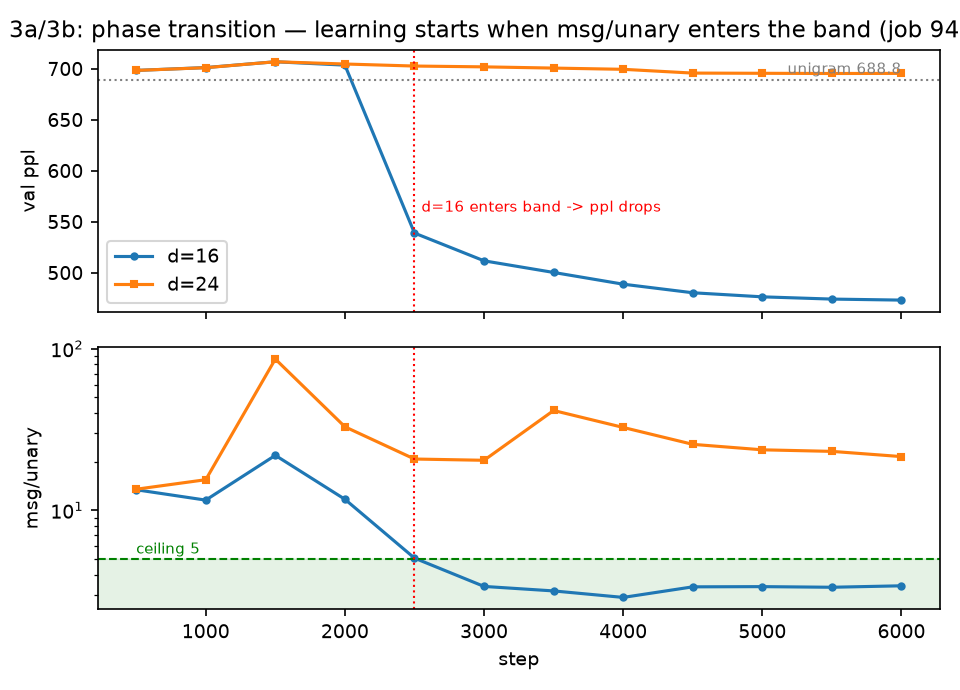
\includegraphics[width=0.86\textwidth]{report_figures/fig1_phase_transition.png}
\caption{The phase transition (job 940844): validation perplexity and \msgu{} on one time
axis, $d{=}16$ vs $d{=}24$. Learning begins at the evaluation where \msgu{} first enters the
band; at $d{=}24$ it never enters and perplexity never leaves the unigram.}
\label{fig:phase}
\end{figure}

\begin{figure}[h]\centering
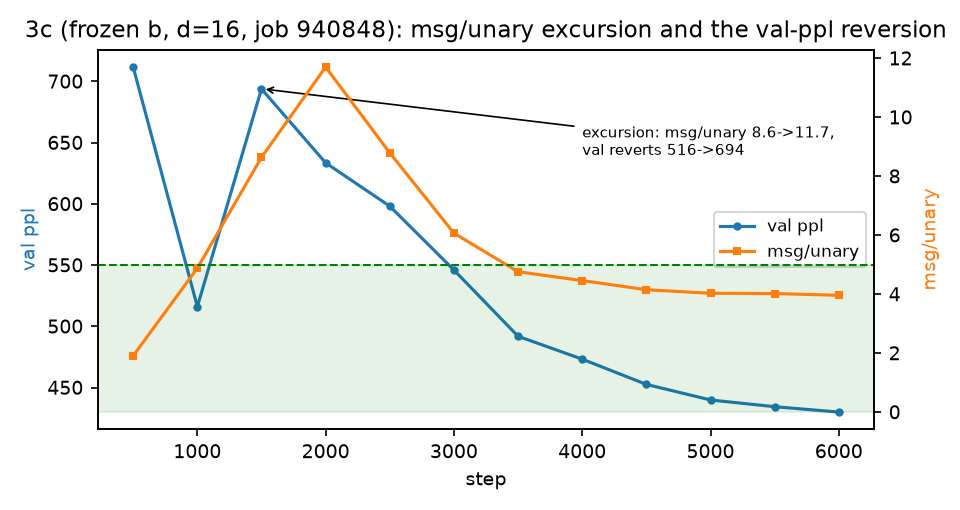
\includegraphics[width=0.86\textwidth]{report_figures/fig2_excursion.png}
\caption{The 3c excursion (job 940848, frozen $b$): \msgu{} leaves the band at steps
1500--2000 and validation perplexity reverts $516 \to 694$, then falls monotonically once
the scalar re-enters --- the two-sided evidence.}
\label{fig:excursion}
\end{figure}

\begin{figure}[h]\centering
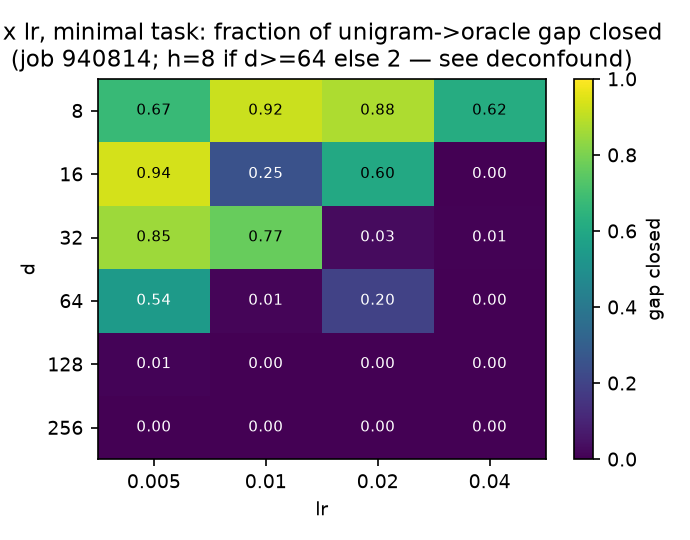
\includegraphics[width=0.6\textwidth]{report_figures/fig3_d_lr_grid.png}
\caption{$d \times \mathrm{lr}$ on the minimal task (job 940814): fraction of the
unigram-to-oracle gap closed.}
\label{fig:dlr}
\end{figure}

\begin{figure}[h]\centering
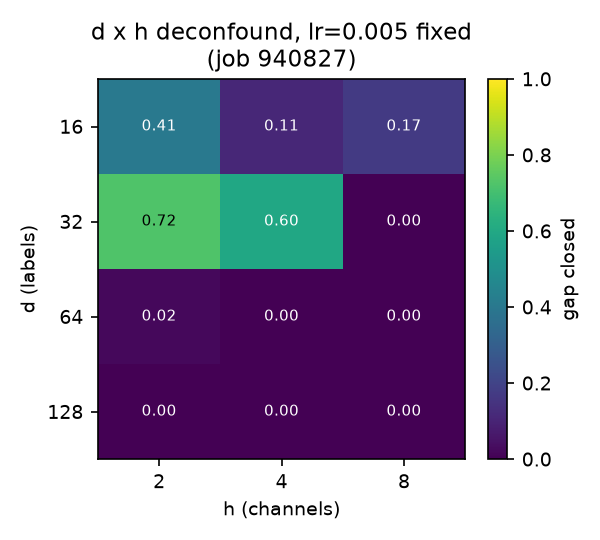
\includegraphics[width=0.55\textwidth]{report_figures/fig4_d_h_deconfound.png}
\caption{$d \times h$ deconfound at fixed lr (job 940827): channels and width degrade the
model independently.}
\label{fig:dh}
\end{figure}

\begin{figure}[h]\centering
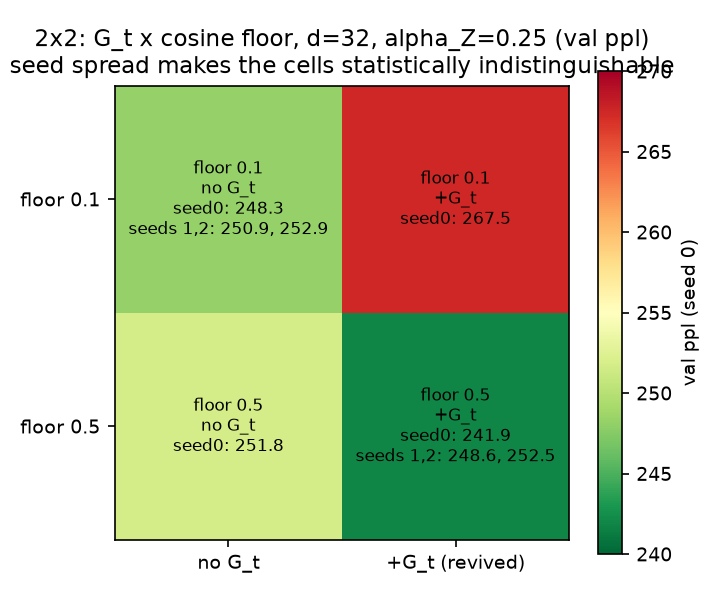
\includegraphics[width=0.6\textwidth]{report_figures/fig5_2x2.png}
\caption{The $G_t \times$ floor square at $d{=}32$, $\alpha_Z{=}0.25$, with seed
replication: the apparent interaction does not survive the seed spread.}
\label{fig:sq}
\end{figure}

\begin{figure}[h]\centering
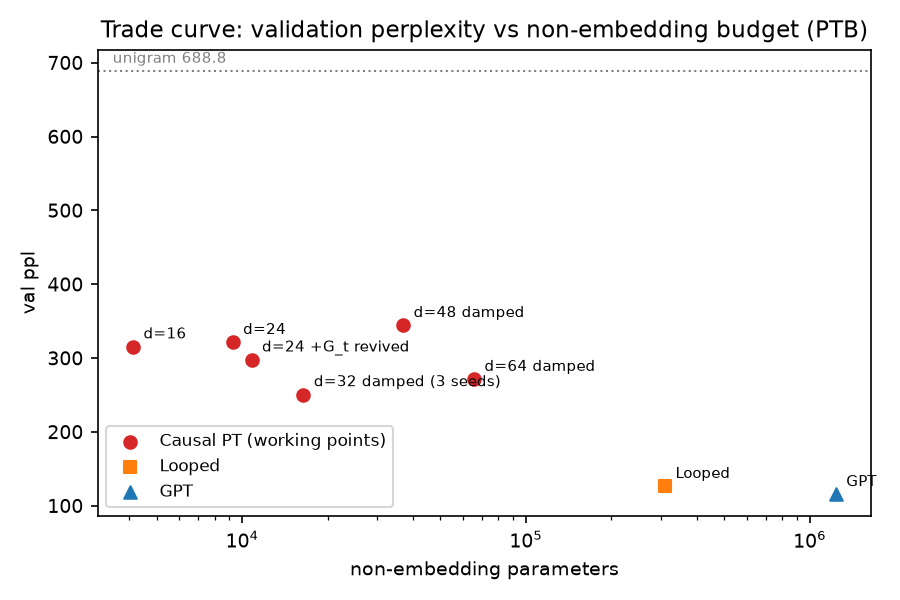
\includegraphics[width=0.8\textwidth]{report_figures/fig6_trade_curve.png}
\caption{Trade curve: validation perplexity vs non-embedding parameters. PT working points
(record with 3-seed error bar), GPT, Looped, unigram line.}
\label{fig:trade}
\end{figure}

\end{document}
